\documentclass[12pt]{article}
\usepackage{amsmath}
\usepackage{graphicx}
\graphicspath{
{images/}  }
\usepackage{caption}
\usepackage{float}
\usepackage[font={small,it}]{caption}
\usepackage{listings}
\usepackage{multicol}
\begin{document}
\title{Hot and Cold Data Storage with PostgreSQL and HBase}
\author{Justin Paul, Sean O'Reilly, Tate Travaglini}
\date{April 29, 2015}
\maketitle

% ------------------------------------------
% Abstract
% ------------------------------------------
\begin{abstract}
When creating applications that use large data sets, developers are often faced with a choice. They can either choose a data storage system that can be accessed quickly or one that scales well. For many developers with limited resources, they cannot have the best of both worlds. 

Data that needs to be accessed quickly is often referred to as “hot data”. When building a system that accesses a large dataset, certain subsets of that data tend to be accessed more often. This set of hot data stands in contrast to cold data; cold data is the large subset of data that rarely needs to be accessed. This data is most often accessed in aggregation over a large portion in order to address longer-term business needs and analytics.
\end{abstract}

% -------------------------------------------
% INTRODUCTION
% -------------------------------------------
\section{Introduction}
Separating the storage of hot and cold data can help solve the issue of choosing between a system where data can be accessed quickly and one that scales well. Traditionally, companies have used different storage media in order to separately store hot and cold data. The hot data would live in fast-access memory, while the cold data would be transferred to longer-term storage media such as magnetic tapes or, more recently, optical disks. However, this solution presents an obvious problem; in order to access the cold data, an administrator will have to physically access the magnetic tape and transfer the data over to a hard drive such that the data could be read. This time consuming data transfer process introduces significant costs and inefficiencies into the system. 


Our solution takes a different approach; we have combined a traditional RDBMS system with a NoSQL column-oriented key-value store. RDBMSs have long been the standard when it comes to real-time querying of data, and for good reason; years of development effort have led to query optimizers and other developments that can very quickly return the data for a user-specified queries. These systems are ideal for storing hot data since, when the amount of data stored is low, they can provide real-time query response performance. NoSQL, on the other hand, is very well suited for cold data storage. By using column-oriented storage, these systems are able to more easily compress the data and easily scale to huge data storage needs while providing efficient aggregated-data querying. However, this scaling ability comes at a cost- these systems often have slow user-specified query response times.
We remedied this problem by creating a user friendly, web-scale system that allows developers to access their data in an agile and scalable fashion. Our system combines a RDBMS with a scalable, NoSQL, column-oriented data store. The system exchanges data between these two different data storage schemes such that the hot data remains in the RDBMS while the cold data remains in the more scalable column-store.


% -------------------------------------------
% Programming Model
% -------------------------------------------
\section{Programming Model}
This system creates two separate database management systems. These DBMS’s can use whatever implementation behind the scenes but are queried by the user using simple key/value pairs.

\subsection{API}
The systems API consists of a way constructor to initialize the DBMS and then hooks to interact with the data. We implemented these in our design; however, if the user wishes to use a different DBMS they simply configure their API to use these hooks. The hooks are defined as follows in pseudo-code:
\begin{lstlisting}[
    basicstyle=\small
]

load(String tableName, List<Map> dataList):
    //Load each piece of data from dataList
    //into table name tableName
    //inserts only into cold storage

scan(String tableName):
    //scans cold storage for every piece 
    //of data in the cold storage

insert(String tableName, Map data):
    //insert data into table named tableName
    //inserts into both hot and cold storage

query(String tableName, String key, List<String> cols):
    //return columns from tableName at key
    //if data not in hot storage pulls it into hot storage

delete(String tableName, String key):
    //deletes key from both hot and cold storage

update(String tableName, String key, Map data):
    //updates data at key in tableName with data
    //writes to both hot and cold storage

\end{lstlisting}

\subsection{Data Structure}
Even though one or both of the DBMS used may allow for unstructured data (as we will later see with our implementation using HBase), this system requires that all tables be initialized with a specific structure that cannot change throughout the lifecycle of the table. This design decision was made to ensure that the system could handle a wide variety of DBMS implementations and was not limited to just NoSQL systems that provide support for unstructured data. 
Again, even though one or both of the DBMS may not necessarily be designed to work as simple key value pairs, the user still interacts with the system through those pairs. If the system does use a DBMS that does not use key/value pairs explicitly, the programmer is required to configure the DBMS in a way that allows these to be used. We will explain how this can be done in more detail in the implementation section. This design decision was made again to support a wide variety of DBMS. By using key/value pairs instead of tuples, nearly any DBMS can be plugged into our system and with minor  modifications work seamlessly.

\section{Implementation}
When we created our implementation of this system we choose to use PostgreSQL to store hot data and Apache HBase to store cold data. Although many different choices can be used, we choose these two DBMS because we felt like developers always are pressured to choose between SQL and NoSQL. We also found that for small datasets SQL is extremely fast, but for larger more web scale problems, NoSQL works better. By marrying these two systems we hoped to create a system with less compromises optimized for read performance.

\subsection{Execution Overview}
When creating an instance of this System, the user specifies a name to be used for both the PostgreSQL and HBase instances and then initializes any tables they plan on using. Finally, they specify a replacement algorithm to be used to swap between hot and cold storage. The user can then use any of the hooks to load and query data. 

\subsubsection{Load}
Since most loads are quite large we did not want our system wasting time updating the hot storage only to swap out newly loaded data. For this reason we decided to load straight into HBase using simple batch puts.

\subsubsection{Insert}
Inserts on the other hand are intended to be smaller in size, usually only a few at a time. These are also intended to be records that the user plans on using soon so these are loaded both into PostgreSQL and HBase. The write into HBase is done again using a simple put on the key but the write into PostgreSQL is a bit more complicated because it is not designed as a key/value store. We decided to simply store the key as a column in PostgreSQL so we could use PostgreSQL with our standard hooks. 

\subsubsection{Query}
Queries first check if the key being queried is in PostgreSQL and, if it is, does a simple select for the specified columns on the table where the key = input key. If not, the system queries HBase for the whole row, writes the entire row of data into PostgreSQL and then returns the specified rows from the data retrieved from HBase. 
We had to make an obvious tradeoff between consistency and performance when designing our query implementation. Idealy, if the data was not in hot storage we would simply query HBase for the specified columns and then return those to the user. The problem we faced was that we would then be unable to load that row into PostgreSQL and take advantage of locality without sacrificing consistency between hot and cold storage. We decided we would rather have consistency for two reasons:

\begin{enumerate}
  \item It makes the system easier to reason about because you know if you query data you are always getting a complete record
  \item If a user queries some specific columns in a row, the principle of locality states that they may not just use those columns again but they may also use any other columns in that row. As a result, loading the entire row into hot storage provides better performance for later queries.
\end{enumerate}

\subsubsection{Delete}
Deletes are implemented doing a simple check on PostgreSQL, deleting if present and then deleting in HBase. 

\subsubsection{Update}
Updates first do a check to see if the data is in PostgreSQL. If it is, it updates the required columns in both PostgreSQL and in HBase. If not, it updates the required fields in HBase and then writes the entire row into PostgreSQL. We had to make a similar design decision like we made when implementing query about the tradeoffs between consistency and performance. For similar reasons, we choose to write the entire row into PostgreSQL instead of just writing the updated rows.

\subsection{Read vs Write Focus}  
Careful readers may be questioning a huge design decision made in regards to the implementation of insert and update when the data is already in PostgreSQL. It seems like those methods could have their performance increased drastically by not writing to HBase and instead writing all updates when those records need to be swapped out. While this implementation would certainly increase the speed of writes, reads would then need to perform an extra write to HBase if the data was not in PostgreSQL. As our system is designed to be a read optimized system, we felt that this overhead was unacceptable and thus decided to implement writes the way we did. 

\subsection{Replacement Algorithms}
The implementation of the Hot and Cold system is adaptable for varying situations. In order to find optimal solutions for the range of uses, a number of different algorithms were explored for the replacement of hot data when hot data storage was full. The replacement algorithms mirror those for page replacement algorithms, namely first-in first-out, clock, random, and least recently used.

\subsubsection{First in, first out (FIFO)}
   
\begin{figure}[h]
\centering
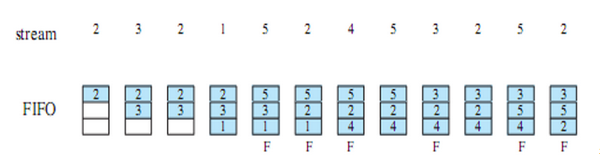
\includegraphics[width=\columnwidth]{FIFO}
\caption{Figure 1: Example of FIFO replacement \cite{10}}
\end{figure}

Replacement with first-in, first-out (Figure 1) keeps track of data using a queue data structure. The newest data is appended to the end of the queue, and the oldest data is at the front of the queue. When the queue is full and new data is needed to be inserted, the oldest data at the front of the queue is removed to make room for the new data which is appended to the end of the queue. The previously second oldest data is now at the front of the queue as the now oldest data. Even with an access to data that is already in the queue, the data is moved to the end of the queue. While this replacement algorithm contains little overhead, it typically exhibits poor performance in page replacement.

\subsubsection{Clock: Static vs Dynamic}
   
\begin{figure}[h]
\centering
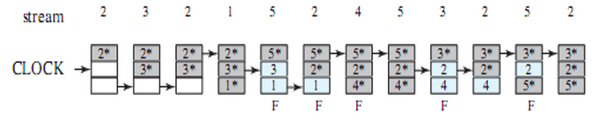
\includegraphics[width=\columnwidth]{Clock}
\caption{Figure 2: Example of Clock replacement \cite{10}}
\end{figure}

This system contains two versions of the clock replacement algorithm; the first clock replacement algorithm is a static version, and the second is a dynamic version. The generalized version of the clock algorithm is seen in Figure 2. In general, each data element in the clock algorithm’s data structure has an extra bit called the referenced bit. Additionally, the clock’s data structure contains an iterator named the hand which points to the last inspected data. Inspection occurs when data is inserted. When this algorithms data structure is not full, appending occurs as usual. When the structure is full, the hand checks the data it currently points to. If the data contains a referenced bit, it is cleared and the hand moves to the next data element. If the data does not have a referenced bit, that data is removed and replaced with the new data, which is given a referenced bit. If data that is already in the data structure is accessed, a referenced bit is given if no referenced bit is connected to the data presently.
        The two versions used in this system differ in their static and dynamic memory management in their data structure. In the static implementation, the data structure size is a constant max size while the dynamic implementation has a varying size. Both versions were utilized in order to find deeper insight into the efficiency of deletions from hot and cold storage. Deletions in the static version remove the data and mark the space as empty for new data insertions. Deletions in the dynamic version remove the data and the memory space it takes up; new data is then appended. Conventionally, the general clock replacement algorithm is more efficient than first-in, first out replacement algorithm.

\subsubsection{Least Recently Used (LRU)}
   
\begin{figure}[h]
\centering
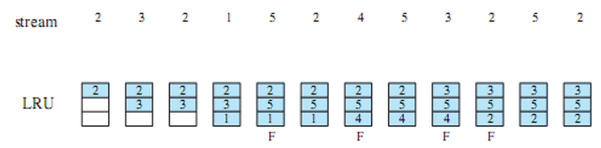
\includegraphics[width=\columnwidth]{LRU}
\caption{Figure 3: Example of LRU replacement \cite{10}}
\end{figure}

A more expensive replacement algorithm is least recently used (Figure 3). The basis of least recently used is the data that has been most heavily utilized recently will be the data that is most utilized in the near future. Thus, when the least recently used data structure is full and needs to replace data, the data that is the coldest, or that which has not been accessed for longest period of time, is removed and replaced with the new data. In this system, implementation of least recently used is controlled by a priority queue; timestamps regulate the ordering of the priority queue. If data in the priority queue is accessed, its timestamp is updated instead of the data being removed from the structure. The least recently used replacement algorithm coincides with the principle of locality and is considered as one of the closest replacement algorithms to optimal efficiency.

\subsubsection{Optimal}
   
\begin{figure}[h]
\centering
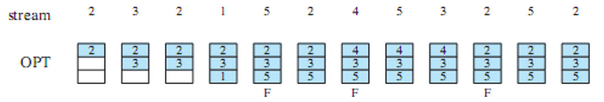
\includegraphics[width=\columnwidth]{Optimal}
\caption{Figure 4: Example of Optimal Replacement \cite{10}}
\end{figure}

The optimal replacement algorithm is a theoretical replacement algorithm where you always make the most intelligent choice for replacement. It requires full knowledge of queries and to get the optimal replacement strategy takes exponential time. The optimal is mainly used for comparison purposes to see how good other algorithms perform.

\subsubsection{Random}
Random replacement works, as the name suggests, by simply choosing a random record to swap out. 

\section{Evaluation}
This section describes the results of testing the performance of our Hot and Cold Data Storage System. In order to test our system, we used the workload from the TPC-W benchmark. Since one of our stated goals is to build a web-scale database system, TPC-W seemed like an obvious choice; the benchmark is designed to test an e-Commerce workload. Specifically, the benchmark is designed to simulate a website that is selling books to customers. The workload is such that it will allow us to analyze the system’s response to storing both hot and cold data. The use of this general purpose benchmark enables us to draw fair comparisons between the performance metrics gathered from each of the tested configurations. We ran our system tests on a 5.8 million row table. Reads ran with 100 thousand queries and writes ran with 50 thousand inserts and 50 thousand updates for a total of 100 thousand queries.

\subsection {Performance}
Besides the traditional sequential read, sequential write, random read and random write benchmarks, we also included another benchmark: random reads with good locality. We defined ‘good locality’ as queries that use 0.1\% of the total data. As this system was designed to perform well for random reads with ‘good locality’ we believed this to be the most interesting metric. We compared each metric to a pure HBase solution.

\subsubsection{Random Write}
Random writes performed the worst of all other metrics resulting in a whopping 6x decrease in performance over HBase. Although this number is eye popping the result is expected as this system is required to perform at worst a PostgreSQL delete and write plus a write to HBase. 

\subsubsection{Sequential Write}
Sequential writes are implemented to only write to cold storage so the sequential write tests produced no increase or decrease in performance over HBase. 

\subsubsection{Random Read}
Completely random reads saw a moderate 2x decrease in performance. Without good locality, the system incurs overhead from swapping in and out of hot storage without significant enough amounts of hits. 

\subsubsection{Random Read with Good Locality}
The random read with good locality produced the best results when compared to HBase. With optimal hot storage size and optimal replacement algorithm we produced a 43\% increase in performance over HBase. 

\subsubsection{Sequential Read}
Like sequential writes, sequential reads are implemented to just scan cold storage so there was no increase or decrease in performance over HBase.


\subsection{Optimal Hot Storage Size}

\begin{center}
  \begin{tabular}{ | l | c |}
    \hline
    Hot-Data Size & Performance Increase \\ \hline \hline
    1\% & 20\% \\ \hline 
    2\% & 25\% \\ \hline
    10\% & 43\% \\ \hline
    50\% & 30\% \\ \hline
    100\% & 15\% \\
    \hline
  \end{tabular}
\end{center}

We ran all of our tests on a system with varying hot storage size ranging from 1\% to 100\% of ‘good locality data.’ We ran these tests holding the replacement algorithm constant (using Least Recently Used). Our results showed that the optimal size of hot storage is 10\% producing the best results in all metrics. 

\subsection{Optimal Replacement Algorithm}

\begin{center}
  \begin{tabular}{ | l | c |}
    \hline
    Replacement Algorithm & Performance Increase \\ \hline \hline
    FIFO & 21\% \\ \hline 
    LRU & 39\% \\ \hline
    Clock 1 & 29\% \\ \hline
    Clock 2 & 42\% \\ \hline
    Random & 5\% \\
    \hline
  \end{tabular}
\end{center}

We also ran all of our tests holding the hot storage size constant (at 10\% of ‘good locality data’) and varied the replacement algorithm. We discovered that the Clock 2 replacement algorithm produces the best results. Even though it has the most overhead, it produces swaps that are closest to optimal resulting in significantly more hits and better performance overfall.

\section{Future Work}
There are many aspects of this system that we were unable to complete and would like to add to the system. The first is a more verbose querying interface so that user can perform more complex operations besides just getting and setting data. To do this we hope to use Apache Phoenix so that a user’s SQL query could be used for both PostgreSQL and HBase. Additionally we hope to add support for an Object Relational Mapping so users can interact directly with objects instead of writing long SQL queries. 
The second this we would have liked to work on is experimenting with DBMS for hot and cold storage. We chose PostgreSQL and HBase because we were familiar with both of them but different DBMS could have produced better performance.

\section{Conclusion}
This work has shown us that for very niche workloads, a hybrid system of HBase and PostgreSQL can produce better performance than just standard HBase. If the workload is majority loads or reads with good locality then our hybrid produces a non-negligible speed up. This research has shown us that hybrid systems like this are not only possible but also plausible replacements for certain data sets. 

\section{Related Work}
There have been a number of other groups that have worked on various types of data storage optimizations for hot vs. cold data. Levandoski et al. explored identifying the sets of hot versus cold data for a main-memory OLTP system being developed by Microsoft codenamed Hekaton. Their work focused on researching classification algorithms that could efficiently identify which data should be classified as hot storage vs. cold storage\cite{1}. In a similar paper titled Trekking Through Siberia: Managing Cold Data in a Memory-Optimized Database, Eldawy et al. explore how a framework called Siberia is implemented. The focus of the paper is describing how Siberia handles transferring data from the Hekaton main-memory database to cheaper secondary storage in a transactionally consistent manner\cite{2}. Höppner et al. studied how to vertically partition data into hot and warm data in order to optimize memory access times for hybrid-memory data storage systems that include both DRAM and a SSD\cite{3}. DeBrabant et al. researched a cold data migration scheme known as anti-caching for use with H-Store\cite{4}. However, unlike our work, the focus of their work is on moving data from a main-memory store database to disk in a transaction-safe manner as the database grows.
Other groups have explored combining together aspects of a RDBMS with a NoSQL system, also known as polyglot persistence. A number of useful guides have emerged that cover the entire spectrum of when and how to use polyglot persistence for more efficient data storage and access\cite{5},\cite{6}. A specific example of one of these implementations is Craigslist. Government regulations require that Craigslist maintains a digital record of their classifieds. With hundreds of thousands of new classifieds being listed per day, maintaining this archive using a RDBMS would prove nearly impossible. As such, Craigslist adopted a model where the more active classifieds are stored in MySQL while the archived data is transferred over to MongoDB\cite{7}. 

Apache Sqoop is a tool designed by the Apache Software Foundation that helps enable the transfer of bulk data between Hadoop and structured database systems such as RDBMSs\cite{8}. Unlike our system, this tool is not meant to perform at interactive speeds; it is built primarily for large, bulk loading jobs. 

In class, we studied HadoopDB, an architectural hybrid of MapReduce and RDBMS technologies\cite{9}. However, HadoopDB differs from our system in that HadoopDB uses Hadoop as a database coordinator that enables communication between multiple PostgreSQL instances. In our system, the data is actually stored in both the NoSQL system and the RDBMS instance. 


\begin{thebibliography}{9}

\bibitem{1}
  Justin Levandoski, P-A Larson, and Radu Stoica
  \emph{Identifiying hot and cold data in main-memory databases},
  Data Engineering(ICDE), 2013 IEE 29th International Conference 
  on 8 APR. 2013: 26-37

\bibitem{2}
  Ahmed Eldawy, Justin Levandoski, and Paul Larson
  \emph{Trekking through siberia: Managing cold data in a memory-optimized database}, Proceedings of the VLDB Endowment 7.11 (2014).

\bibitem{3}
  Bernhard Höppner, Ahmadshah Waizy, and Hannes Rauhe
  \emph{An approach for hybrid-memory scaling columnar in-memory databases}, Proceedings of the VLDB Endowment 7.14 (2014).

\bibitem{4}
  Justin DeBrabant
  \emph{Anti-caching: A new approach to database management system architecture}, Proceedings of the VLDB Endowment 6.14 (2013).

\bibitem{5}
  \emph{Data Access for Highly-Scalable Solutions: Using SQL ...}, 2015. 29 Apr. 2015 

\bibitem{6}
  \emph{Introduction to Polyglot Persistence: Using Different Data ...}, 2012. 29 Apr. 2015 

\bibitem{7}
  \emph{Craigslist Customer Success with MongoDB | MongoDB}, 2013. 29 Apr. 2015 

\bibitem{8}
  \emph{Sqoop - - The Apache Software Foundation!}, 2012. 29 Apr. 2015

\bibitem{9}
  Azza Abouzeid
  \emph{HadoopDB: an architectural hybrid of MapReduce and DBMS technologies for analytical workloads}, Proceedings of the VLDB Endowment 2.1 (2009)

\bibitem{10}
  William Stallings
  \emph{Operating Systems: Internals and Design Principles}

\end{thebibliography}
\end{document}
